\documentclass[a4paper,12pt]{article}

% --- Paketi ---
\usepackage[utf8]{inputenc}
\usepackage[T1]{fontenc}
\usepackage[slovene]{babel}
\usepackage{lmodern}
\usepackage{amsmath, amssymb}
\usepackage{amsthm}
\usepackage{graphicx}
\usepackage{url}

% --- Okolja za definicije, izreke, dokaze ---
\theoremstyle{definition}
\newtheorem{definicija}{Definicija}

\theoremstyle{plain}
\newtheorem{izrek}{Izrek}

% Nastavitve razmikov
\setlength{\belowcaptionskip}{2mm}
\setlength{\parindent}{0mm}

% --- Glava dokumenta ---
\title{Magični kvadrati}
\date{} % (1. naloga) odstranimo datum

\begin{document}

\maketitle

%%%%%%%%%%%%%%%%%%%%%%%%%%%%%%%%%%%%%%%%%%%%%%%%%%%%%%%%%%%%%%%%%%%%%%%%
% 2. naloga – vključitev slike
%%%%%%%%%%%%%%%%%%%%%%%%%%%%%%%%%%%%%%%%%%%%%%%%%%%%%%%%%%%%%%%%%%%%%%%%

\begin{center}
    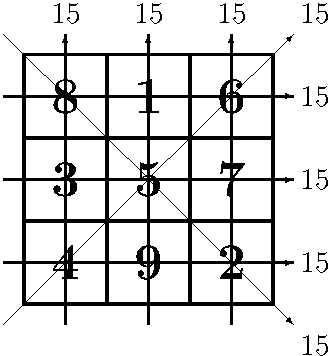
\includegraphics[width=0.8\textwidth]{slika.pdf}
\end{center}

Prirejeno iz virov:

%%%%%%%%%%%%%%%%%%%%%%%%%%%%%%%%%%%%%%%%%%%%%%%%%%%%%%%%%%%%%%%%%%%%%%%%
% 3. naloga – spletni naslovi z \url
%%%%%%%%%%%%%%%%%%%%%%%%%%%%%%%%%%%%%%%%%%%%%%%%%%%%%%%%%%%%%%%%%%%%%%%%

\begin{itemize}
   \item \url{http://mathworld.wolfram.com/MagicSquare.html}
   \item \url{http://en.wikipedia.org/wiki/Magic_square}
\end{itemize}

%%%%%%%%%%%%%%%%%%%%%%%%%%%%%%%%%%%%%%%%%%%%%%%%%%%%%%%%%%%%%%%%%%%%%%%%
% 4. naloga – kazalo vsebine
%%%%%%%%%%%%%%%%%%%%%%%%%%%%%%%%%%%%%%%%%%%%%%%%%%%%%%%%%%%%%%%%%%%%%%%%

\tableofcontents

\newpage
%%%%%%%%%%%%%%%%%%%%%%%%%%%%%%%%%%%%%%%%%%%%%%%%%%%%%%%%%%%%%%%%%%%%%%%%
% 5. naloga – definicije in tabele
%%%%%%%%%%%%%%%%%%%%%%%%%%%%%%%%%%%%%%%%%%%%%%%%%%%%%%%%%%%%%%%%%%%%%%%%

\section{Uvod}

\begin{definicija}
\emph{Magični kvadrat} reda $n$ je nabor $n^2$ različnih števil,
ki so razvrščena v kvadratno tabelo tako, da vedno dobimo enako vsoto,
če seštejemo vsa števila poljubne vrstice, stolpca ali katere koli glavne diagonale.
\end{definicija}

Primer magičnega kvadrata reda 3 je prikazan v tabeli~\ref{table:mag3}.

\begin{table}[h!]
   \centering
   \caption{Magični kvadrat reda 3}
   \label{table:mag3}
   \begin{tabular}{|c|c|c|}
      \hline
      8 & 1 & 6 \\ \hline
      3 & 5 & 7 \\ \hline
      4 & 9 & 2 \\ \hline
   \end{tabular}
\end{table}

\begin{definicija}
Magični kvadrat reda $n$ je \emph{normalen}, če v njem nastopajo števila
\begin{equation}
   \label{eq:numbers}
   1, 2, 3, \ldots, n^2.
\end{equation}
\end{definicija}

Magični kvadrat v tabeli~\ref{table:mag3} je normalen.
To je tudi najmanjši netrivialen normalen magični kvadrat.

%%%%%%%%%%%%%%%%%%%%%%%%%%%%%%%%%%%%%%%%%%%%%%%%%%%%%%%%%%%%%%%%%%%%%%%%
% 6. naloga – izreki in dokazi
%%%%%%%%%%%%%%%%%%%%%%%%%%%%%%%%%%%%%%%%%%%%%%%%%%%%%%%%%%%%%%%%%%%%%%%%

\section{Osnovne lastnosti}

\begin{definicija}
Vsoto ene vrstice, enega stolpca ali ene od glavnih diagonal
v magičnem kvadratu imenujemo \emph{magična konstanta}.
\end{definicija}

\begin{izrek}
Magična konstanta normalnega magičnega kvadrata reda $n$ je enaka
\begin{equation}
   \label{eq:mc}
   M_2(n) = \frac{1}{2} n (n^2 + 1).
\end{equation}
\end{izrek}

\begin{proof}
V normalnem magičnem kvadratu reda $n$ je vsota vseh nastopajočih
števil (glej~\ref{eq:numbers}) enaka
\[
1 + 2 + 3 + \dots + n^2 = \sum_{k=1}^{n^2} k = \frac{1}{2} n^2 (n^2 + 1).
\]
Ker imamo v kvadratu $n$ vrstic z enako vsoto, je vsota števil v eni vrstici
enaka številu $M_2(n)$.
\end{proof}

\begin{definicija}
Če vsako od števil v normalnem magičnem kvadratu reda $n$ odštejemo
od števila $n^2 + 1$, dobimo nov magični kvadrat, ki je prvotnemu
\emph{komplementaren}.
\end{definicija}

\begin{definicija}
Pravimo, da sta dva magična kvadrata \emph{različna}, če enega ni mogoče dobiti
iz drugega s pomočjo zasukov oziroma zrcaljenj.
\end{definicija}

%%%%%%%%%%%%%%%%%%%%%%%%%%%%%%%%%%%%%%%%%%%%%%%%%%%%%%%%%%%%%%%%%%%%%%%%
% 7. naloga – primer dodatne tabele (opcijsko)
%%%%%%%%%%%%%%%%%%%%%%%%%%%%%%%%%%%%%%%%%%%%%%%%%%%%%%%%%%%%%%%%%%%%%%%%

\section{Primeri}

\begin{table}[h!]
   \centering
   \caption{Magični kvadrat reda 5}
   \label{table:mag5}
   \begin{tabular}{|c|c|c|c|c|}
      \hline
      17 & 24 & 1 & 8 & 15 \\ \hline
      23 & 5 & 7 & 14 & 16 \\ \hline
      4 & 6 & 13 & 20 & 22 \\ \hline
      10 & 12 & 19 & 21 & 3 \\ \hline
      11 & 18 & 25 & 2 & 9 \\ \hline
   \end{tabular}
\end{table}

%%%%%%%%%%%%%%%%%%%%%%%%%%%%%%%%%%%%%%%%%%%%%%%%%%%%%%%%%%%%%%%%%%%%%%%%

\end{document}
